\documentclass[a4paper,oneside,10pt,final]{report} 

% Options possibles : 10pt, 11pt, 12pt (taille de la fonte)
%                     oneside, twoside (recto simple, recto-verso)
%                     draft, final (stade de d�veloppement)

\usepackage[latin1]{inputenc} % LaTeX, comprends les accents !
%\usepackage[T1]{fontenc}      % Police contenant les caract�res fran�ais
%\usepackage{geometry}         % D�finir les marges
\usepackage[francais]{babel}  % liste de langues, la derni�re �tant la langue
                              % principale
\usepackage{graphicx}


% Les param�tres du titre�: titre, auteur, date
\title{ext3Viewer \\ Rapport de projet}
\author{Laurent Sebag \and Nathan Periana \and \\Tuteur:M. Konstantin Verchinine}
\date{2006-2007}

\makeindex

%%%%%%%%%%%%%%%%%%%%%%%%%%%%%%%%%%%%%%%%%%%%%%%%%%%%%%%%%%%%%%%%%%%%%%%%%%%

\begin{document}
\maketitle
\tableofcontents

\newpage

\chapter {Introduction}
\section{Introduction}
L'id�e g�n�rale que l'on se fait souvent d'un syst�me de fichier est celle d'une 
organisation permettant la gestion de deux composants : les fichiers, et les 
dossiers, qui les contiennent. Les syst�mes de fichiers sont utilis�s sur les m�moires secondaires : disques durs, cl�s USB, cd-rom \ldots{}\\

Ce projet tutor� porte sur le syst�me de fichier ext3, tr�s utilis� dans le 
monde de Linux. Ce syst�me de fichier est dit "journalis�", c'est � dire que 
l'on garde trace des actions effectu�es sur le disque\footnote{Pendant le
  moment o� les donn�es sont en cache et pas encore �crites sur le disque,
  pour garder l'int�grit� du syst�me de fichier en cas de panne
  mat�rielle.}. D'un point de vue technique, les objets habituels sont tous
represent�s par un \emph{inode}. L'\emph{inode} est une structure de donn�es
qui va permettre de repr�senter tous les objets que l'utilisateur manipule :
les fichier, les dossiers, les p�riph�riques, les liens, etc.

\section{Description}
Le but du projet ext3Viewer est de permettre l'exploration du syst�me de
fichier � un tr�s bas niveau. \\
Beaucoup d'informations administratives sont contenues dans le syst�me de
fichier. Ces donn�es internes, qui permettent l'organisation et la
pr�servation de l'int�grit� des fichiers, sont cach�es � l'utilisateur normal.
Ext3Viewer est destin� aux �tudiants en informatique ayant des connaissances
sur ext3. Il leur permet d'acc�der � toutes les structure cach�es de leur
partition. Ainsi, ils auront une meilleur compr�hension de la fa�on dont sont
stock�es physiquement les donn�es sur un disque dur utilisant ext3.
\\
Le projet ext3viewer a �t� propos� par M. Konstantin Verchinine; il est
destin� � remplacer le projet e2view, qui sert pendant le cours
d'Architecture, Syst�me et R�seaux sur les syst�mes de fichiers. 
%Il a �t� con�u pour des utilisateurs ayant d�ja des connaissances avanc�es en informatique.


\section{Historique et fonctionnement de ext3}
Le syst�me de fichier ext3 est un syst�me de fichiers journalis�,
majoritairement utilis� par le syst�me d'exploitation Linux; mais il est
�galement compatible avec BSD, et dans une moindre mesure, avec Windows. Il a
�t� introduit en Novembre 2001, dans le kernel 2.4.15, pour remplacer
ext2. L'une des raisons de son succ�s est la r�trocompatibilit� avec ce
dernier: une partition ext2 peut �tre convertie vers ext3, et vice versa; et un syst�me de fichier ext3 peut �tre mont� (utilis�) en ext2, moyennant la perte de certaines fonctionnalit�s.
\\
ext3 est organis� de la fa�on suivante\footnote{Le vocabulaire technique est
  expliqu� dans la partie glossaire.}:\\

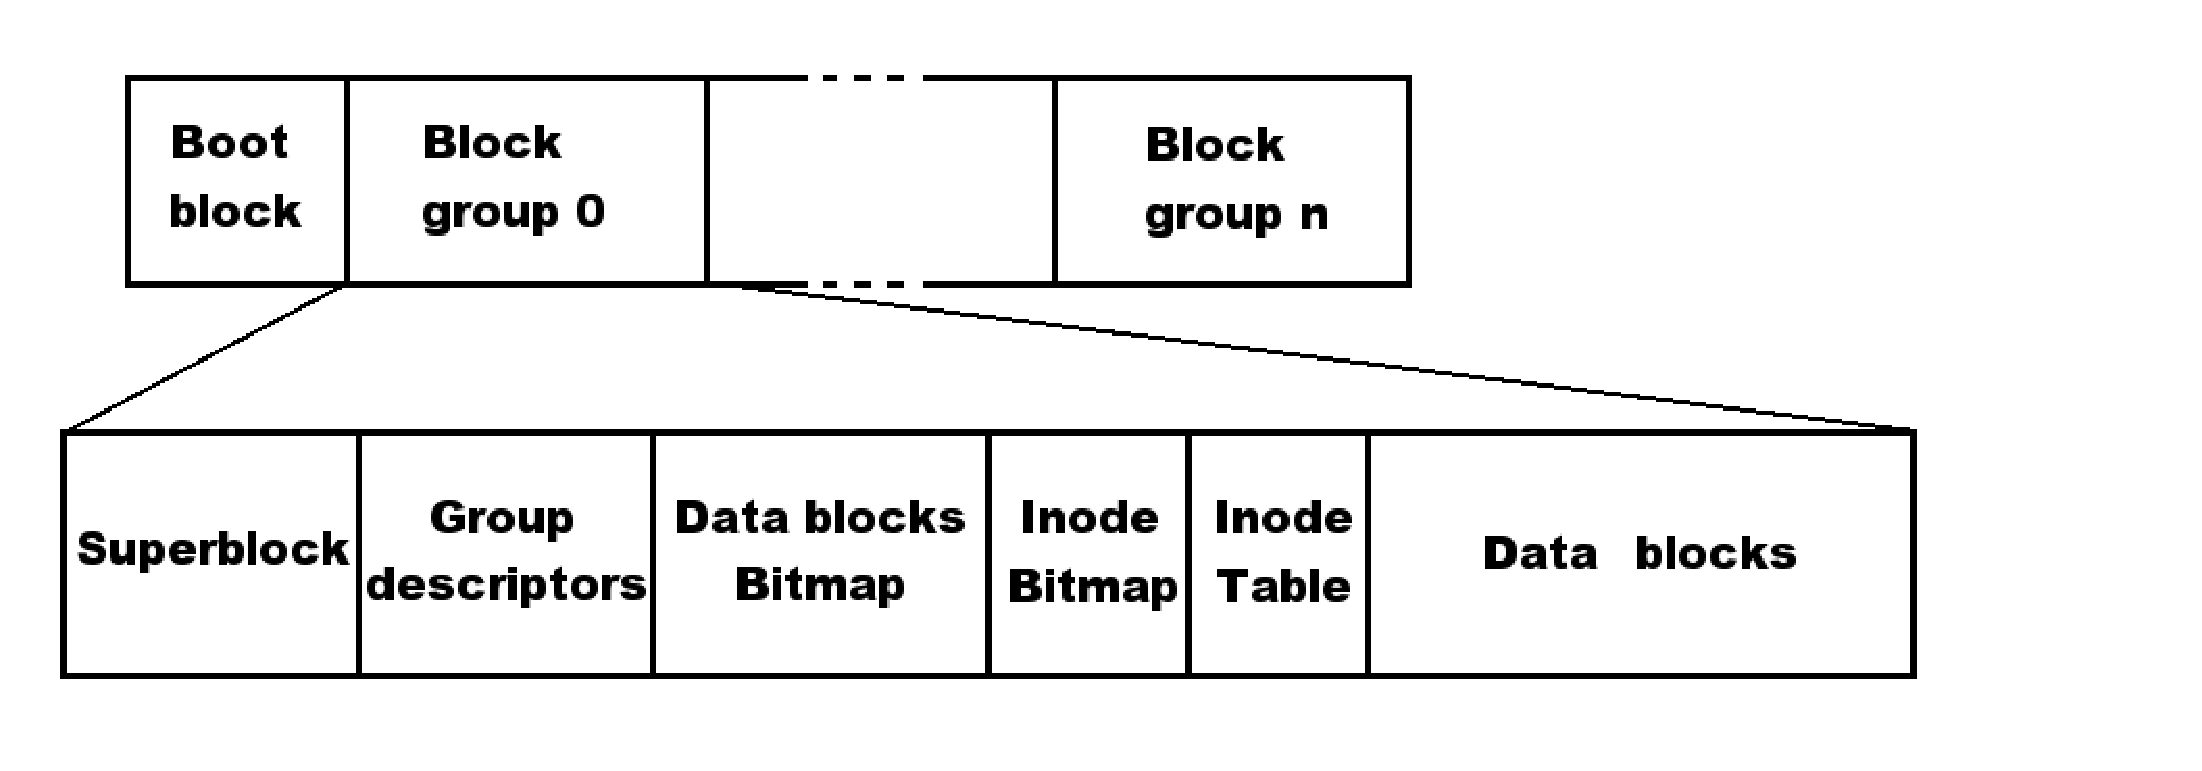
\includegraphics[scale=0.33]{ext3_schema}


Le 'boot block' peut ne pas �tre utilis�, par exemple dans le cas d'un fichier image.
Chaque 'block group' contient une copie du superblock et des group descriptors; mais seuls ceux du premier block group (block group 0) sont utilis�s par le noyau, les autres �tant uniquement des copies de sauvegarde.
L'inode table n'est pas une structure, elle contient simplement l'ensemble des inodes d'un groupe.


\section{Choix pr�liminaires r�alis�s}
Le projet est r�alis� en anglais, comme conseill� par M. Verchinine. Ceci peut
s'expliquer de plusieurs fa�ons: l'anglais est le langage de l'informatique;
le syst�me de fichiers ext3 a donc �t� d�velopp� en anglais, et il n'existe
malheureusement pas de traductions fran�aises officielles pour certaines de
ses fonctionnalit�s.
\\
Il a �t� d�cid� de ne pas se baser sur le projet e2view,pour plusieurs
raisons. D'abord, ce programme �tait pour sa plus grande partie en langue
fran�aise, et les interfaces consoles et graphiques n'�taient pas suffisament
intuitives et ergonomiques; il aurait fallu r��crire une grande partie du code
pour les adapter � nos besoins. Ensuite, le projet ext3viewer se voulait un
moyen de d�couvrir le fonctionnement de ext3; il �tait donc pr�f�rable, d'un
point de vue didactique, de ne pas reprendre un programme d�j� existant.


\chapter {Cahier des charges}
\section{Rappel du cahier des charges}
Le programme devait �tre divis� en deux parties: une partie graphique, et une
partie console.


\subsection*{Fonctionnalit�s utilisateur}

\subsubsection{Visualisation des structures ext3}
	Le programme devait permettre de visualiser les diff�rentes structures du syst�me de fichier ext3 ainsi que les  valeurs prises par chacun des champs, ceux-ci �tant explicit�s. 

\subsubsection{Navigation � travers le syst�me de fichier}
L'interface graphique permettrait de naviguer � travers le syst�me de fichier
tandis que le mode console, r�serv� aux utilisateurs experiment�s, devait
permettre de visualiser les structures. Gr�ce � l'interface graphique,
l'utilisateur devait voir ses fichiers et dossiers habituels et pouvoir
afficher la structure de chaque inode, les informations concernant le \emph{boot
sector}, les \emph{group blocks}, le \emph{superblock}, les \emph{bitmaps}. Le journal du syst�me de
fichier devait �tre affich�. Une explication sur les structures, les
utilisations du syst�me de fichier et leurs cons�quences avait �t� pr�vue pour
une partie aide.
\subsubsection{Correspondance nom/inode et inversement}
Le logiciel pourrait traduire un nom de fichier vers le
num�ro d'inode correspondant, chercher un fichier, � partir
de son num�ro d'inode, et afficher � quel inode est rattach� un block en
tapant son num�ro de block.
\subsubsection{Recherche de structures libres}
Le programme permettrait de trouver le prochain inode libre sur le disque, ou le prochain block libre. On pourrait de plus tester si un inode ou un block est utilis�, et le cas �ch�ant se rendre au bon endroit dans l'arborescence pour afficher la structure du fichier ou dossier.
\subsubsection{Plate-formes d'utilisation}
Le programme serait compatible Linux, et peut �tre Windows et MacOS.

\section{Evolution du cahier des charges}
Comme expliqu� pr�c�demment, le projet a �t� r�alis� en anglais; les modules d'internationalisation n'ont donc pas �t� impl�ment�s.
Le d�coupage mode console/mode graphique a �t� conserv�. Par contre, certaines
fonctionnalit�s n'ont pas �t� d�velopp�es, car elles n'�taient pas
indispensables � la compr�hension g�n�rale de ext3.
Certaines structures, comme les ACLs, n'ont pas �t� affich�es, ou bien affich�es d'une autre fa�on apr�s une �tude plus d�taill�e du syst�me de fichier.\\
La compatibilit� avec Windows a �t� provisoirement abandonn�e, du fait de l'absence de nombreuses fonctions basiques  (open, read, lseek...), mais un port vers cette platforme est th�oriquement possible, en cr�ant ses propres fonctions, en utilisant les fonctions de compatibilit� de la Glib (biblioth�que de Gnome, multiplateforme), ou en utilisant Cygwin...\\
La compatibilit� avec MacOS n'a pas encore �t� test�e, mais est envisageable
(MacOS X est compatible POSIX).
\subsection*{R�sum� des fonctionnalit�s pr�vues/cr��es}

\subsubsection{Visualisation des structures ext3}
OK: Les structures principales sont affich�es, avec des explications suppl�mentaires sur certains de leurs champs. \\
Structures affich�es: \emph{Superblocks, Inodes, Block Bitmap, Inode bitmap,
  Group Descriptors, Journal Superblock Header, Journal Header, Direntries,
  Extended Attributes,Blocks}\\
Structures non affich�es: \emph{Access Control Lists}.

\subsubsection{Navigation � travers le syst�me de fichier}
OK:La navigation est assur�e par un 'explorateur' de fichiers en mode graphique, et par l'option -ls, plus le num�ro d'inode (l'inode de la racine �tant l'inode 2).

\subsubsection{Correspondance nom/inode et inversement}
OK: En mode graphique, l'utilisateur peut y acc�der grace � une barre de
recherche visible sur l'�cran principal; en mode console, il peut y acc�der
grace aux options -find (nom, et num�ro d'inode du dossier parent vers num�ro
d'inode) et -iname (num�ro d'inode vers nom).

\subsubsection{Recherche de structures libres}
OK:Le mode graphique poss�de dans le menu 'Tools' des boutons pour l'affichage
des bitmaps (\emph{inode bitmap},\emph{ block bitmap}), et la recherche du
premier inode ou block libre, pour chaque \emph{block group}.\\
Les fonctions pour d�terminer si un inode ou un block sont utilis�es n'ont pas
�t� d�velopp�es, car l'utilisateur peut aller voir dans l'inode ou le block
bitmap si la structure est occup�e ou non.

\subsubsection{Plate-formes d'utilisation}
Le programme ext3viewer a �t� test� avec Gentoo, SuSe 10.1, Slackware
10.1,11.0 en architecture little-endian. La compatibilit� Windows n'est pas
assur�e, pour la version 1.0. La compatibilit� Mac OS n'a pas �t� test�e.
 Bien que des fonctions du type \emph{le32\_to\_cpu()} soient utilis�es dans le code, pour assurer la compatibilit� avec les machines poss�dant une architecture diff�rente, il faudrait pouvoir la v�rifier directement sur celles-ci.
\\

\chapter {D�veloppement}
\section{Outils employ�s}
Au cours de notre projet, nous avons employ� de nombreux outils; certains tr�s
connus, d'autres moins. Les voici, r�sum�s et d�crits.\\
\begin{itemize}
\item GCC: GCC est le compilateur standard sous Linux.\\
\item Langage C: Le langage C est l'un des langages les plus utilis�s dans le
  code source et dans le monde de Linux. Ext3viewer se positionne donc en
  continuit� avec cette philosophie. \\
\item Le C permet �galement un acc�s bas niveau au disque et � la m�moire,
particuli�rement utiles pour le projet.\\
\item eFence: Biblioth�que Electric Fence, utile pour la v�rification de la
  gestion dynamique de la m�moire. Elle a �t� utilis�e lors de la phase de
  tests, pour d�tecter les erreurs possibles de segmentation fault.\\
\item groff: groff est un outil de formattage, d�di� � la cr�ation de pages
  manuel.\\
\item GTK:Gtk est une biblioth�que graphique, qui a �t� impl�ment�e pour de
  nombreux langages (C, C++, Java, Python...), et de nombreuses platformes
  (Linux,Windows...). Elle a �t� choisie pour son efficacit�, et sa simplicit�
  d'utilisation, ainsi que pour sa disponibilit� sur les machines de l'IUT.\\
\item \LaTeX{}: \LaTeX{} (prononcer 'Latek') est un langage de balises,
  utilis� pour la production des documents, avec une qualit� professionnelle
  (g�n�ration automatique d'index, mise en page, ...).
\end{itemize}

\section{Planning et execution}
\subsection{Planning pr�vu}
\subsubsection{Septembre- fin Octobre:} Planification g�n�rale du projet; cr�ation du planning d�taill�, r�daction d'un cahier des charges.
Dur�e: 1 mois.

\subsubsection{Octobre - mi-d�cembre :} Codage des acc�s au disque, des fonctions de lecture
et des affichages en mode console. Dur�e: 1+1/2 mois 

\subsubsection{Fin d�cembre-fin f�vrier :} Codage de l'interface graphique. R�daction
  d'une partie de l'aide utilisateur. Dur�e : 2+1/2 mois.

\subsubsection{Fin f�vrier - mi-mars :} R�daction du reste de l'aide
utilisateur. R�daction des documentations utilisateur, d�veloppeur, et de la
documentation sur ext3. Cr�ation des fichiers d'internationalisation.



\subsection{Planning effectu� et r�ajustements}


Le planning subi des r�ajustements, en fonction des difficult�s rencontr�es: certaines parties du projet se sont r�v�l�es plus complexes que pr�vues, et certaines ont pris moins de temps. Certaines fonctionnalit�s secondaires ont �t� abandonn�es, pour pouvoir se concentrer sur d'autres plus importantes.\\
En particulier, l'interface console a n�cessit� un travail pr�liminaire d'�tude de ext3; la signification pr�cise des champs des structures et les m�thodes d'acc�s � celles-ci ont dues �tre retrouv�es. Au vu de la nouvelle estimation de la charge de travail, le d�lai fix� pour le d�veloppement du mode console a donc �t� rallong�.\\
L'interface graphique, par contre, a n�cessit� moins de temps que pr�vu, la biblioth�que GTK �tant relativement simple � apprendre et � utiliser.

\subsubsection{Septembre-Octobre}
 Choix et �tude pr�alable du sujet, analyse des besoins, analyse de l'existant, d�finition des fonctionnalit�s n�cessaires, organisation du travail. R�daction du cahier des charges. Dur�e: 1 mois.
\subsubsection{Novembre - mi-d�cembre}
Codage d'une partie du mode console: recherche d'un fichier, correspondance inode/chemin, lecture et affichage du superblock, lecture et affichage des group descriptors, lecture et affichage des direntries (dossiers), lecture et affichage du contenu d'un fichier, lecture et affichage du contenu des blocks, lecture et affichage du contenu d'un inode . Recherche de documentation d�taill�e sur ext3, apprentissage du fonctionnement et de l'organisation de ext3 sur le disque.
\subsubsection{Fin d�cembre-fin f�vrier}
 Codage de l'interface console:
Lecture d'un block en donnant son num�ro, affichage de l'arbre (simplifi�) de l'allocation des blocks pour un inode, affichage du contenu d'un lien symbolique, lecture et affichage des copies du superblock, affichage des blocks indirect comme pointeurs de blocks, lecture et affichage du block bitmap et de l'inode bitmap, affichage du premier block ou inode libre,
Cr�ation de la page manuel, et de l'option d'aide -help (mode console).
D�but de la r�daction des documentations.

\subsubsection{Fin f�vrier - mi-mars} Codage de l'interface console: Lecture et affichage du journal. Affichage des extended user attributes. Nettoyage et r�organisation du code.
Codage de l'interface graphique.
R�daction des documentations utilisateur et d�veloppeur. 
Mise � jour de la page manuel pour refl�ter les changements apport�s au projet.
Tests du programme.
R�daction du rapport.

\subsection{R�partition du travail et m�thodes d'organisation}

\subsubsection{R�partition du travail}
\large
Laurent Sebag\\
\small
\begin{itemize}
\item Cr�ation de l'interface graphique
\item recherche d'un fichier
\item correspondance inode/chemin
\item lecture du superblock
\item lecture et affichage des group descriptors
\item lecture et affichage des direntries (dossiers)
\item lecture et affichage du contenu d'un fichier
\item lecture et affichage du contenu des blocks
\item lecture du contenu d'un inode
\item Lecture d'un block en donnant son num�ro
\item Lecture et affichage du journal
\item conversion d'un nom de fichier vers un num�ro d'inode
\item affichage de l'arbre (simplifi�) de l'allocation des blocks pour un inode
\item affichage du contenu d'un lien symbolique
\item lecture et affichage des copies du superblock
\item affichage des blocks indirect comme pointeurs de blocks
\item Recherche de documentation d�taill�e sur ext3
\item R�daction du cahier des charges
\item R�daction de la documentation utilisateur
\item R�daction de la documentation d�veloppeur
\item R�daction d'une partie du rapport
\item R�daction de la page manuel
\item Tests du programme
\item Coordination du travail
\end{itemize}
\large
Nathan Periana\\
\small
\begin{itemize}
\item affichage et explication du superblock
\item affichage et explication  du contenu d'un inode
\item Recherche de documentation d�taill�e sur ext3 
\item lecture et affichage du block bitmap
\item lecture et affichage  de l'inode bitmap
\item affichage du premier block libre
\item affichage du premier inode libre
\item Lecture et affichage du journal
\item Lecture et affichage des extended user attributes
\item R�daction du cahier des charges
\item R�daction d'une partie de la documentation utilisateur
\item R�daction d'une partie de la documentation d�veloppeur
\item Correction de la page manuel
\item Tests du programme
\item R�daction du rapport
\end{itemize}
\normalsize
\subsubsection{M�thodes d'organisation}
Les fonctionnalit�s � impl�menter �taient regroup�es dans une 'TODO list', qui �voluait au cours du projet; elles �taient attribu�es � un d�veloppeur, et marqu�es comme '� faire',  'effectu�es' ou 'abandonn�es'.\\
Du fait de la petite taille du projet (2 personnes), le syst�me de CVS n'a pas
�t� utilis�. Plusieurs techniques manuelles ont tout de m�me �t� utilis�es
pour le remplacer. Chaque d�veloppeur travaillait sur ses fichier en local, en
essayant d'�viter de modifier simultan�ment le m�me code source. Dans les cas
o� les deux sources �taient modifi�es en m�me temps, l'un des d�veloppeurs se
chargeait de fusionner les codes sources, avec l'aide de l'utilitaire tkdiff
(une interface graphique � l'utilitaire diff, qui compare deux fichiers ligne
par ligne). Le transfert des fichiers se faisait par mail, et la communication
par messagerie instantan�e.

\section{Difficult�s rencontr�es} %cette partie m�rite une section.
L'une des difficult�s majeures rencontr�es dans ce projet est le manque de
documentation technique sur certaines structures. En effet, les documents
trouv�s sur internet concernent majoritairement ext2; bien que les deux
syst�mes de fichiers partagent de nombreuses structures, certaines poss�dent
des diff�rences importantes, ou sont totalement sp�cifiques � ext3.\\
Deux structures ont pos� particuli�rement probl�me: le journal, et les ACL.\\
Deux structures ont pos� particuli�rement probl�me: le journal, et les ACL.
Le journal est g�r� par une couche applicative cr��e pour �tre distincte de
ext3: le JBD (Journaling Block Device). La documentation sur le fonctionnement
de l'API du JBD existe; par contre, son impl�mentation sur le disque n'est que
partiellement visible, dans les 'includes' de d�veloppement.
Les diff�rents champs des
structures sont indiqu�s, mais peu comment�s, et la position des structures
elles-m�mes sur le disque a du �tre 'devin�e', par des tests et par la
consultation des sources de l'utilitaire 'debugfs', qui affiche quelques
informations sur le journal.\\
La documentation concernant les Access Control Lists pose un probl�me similaire, il renseigne sur le fonctionnement g�n�ral de celles ci, mais pas sur leur organisation sur le disque; de plus, les ACL changent selon les versions du noyau.
En effet, les ACL faisaient l'objet d'une sp�cification POSIX, mais elle a �t�
abandon�e; les ACLs sont impl�ment�es diff�rement entre les versions 2.4.28 et
2.6.10+.\\
La programmation de l'acc�s au disque a �galement g�n�r� des complications. En
effet, l'API disponible avec ext3 s'est r�v�l�e inadapt�e aux besoins du
projet; elle ne pouvait fonctionner que sur un syst�me mont�. Le projet, pour
des raisons de coh�rence des donn�es lues et de simplicit� d'utilisation,
devait �tre capable de travailler avec des images ou des disques d�mont�s; il
a donc �t� n�cessaire de cr�er toutes les fonctions d'acc�s au disque.\\


\chapter {Bilans}
%\section*{Bilans personnels}
%Ce tag est n�cessaire seulement si on ajoute un bilan g�n�ral...

\subsection*{Laurent Sebag}


Ce projet m'a permis d'apprendre � r�partir les taches d'un projet entre
plusieurs personnes. Pour cela j'ai utilis� le principe des todo lists :  �
p�riode r�guli�re, je fixait des objectif � atteindre.

J'ai appris � utiliser une API graphique permettant la creation de fen�tres :
gtk+-. Cependant cela m'a fait r�fl�chir sur l'utilisation du c++ ou
d'un autre language orient� objet. Ce serait plus apropri� pour r�aliser une 
interface graphique. 

Gtk simule le concept d'objet, ce qui rend le codage plutot lourd car utilise
des macros pour cela. C'est pourquoi ce projet m'a donn� envie d'essayer gtkmm,
la version de gtk en C++.

Durant le projet j'ai aussi appris � utiliser vim qui est une formidable alternative � emacs : je la conseille car elle comporte des fonctionalit� pratiques pour le codage. L'utilisation de \LaTeX{} est tr�s utiles aussi, le fait de donner l'
organisation d'un texte et qu'il produise en retour un document bien pr�sent� est agr�able.

L'�tudes de parties de codes du noyau et de debugfs m'ont aussi fait r�fl�chir
sur l'organisation des fichiers sources dans un projet. L'utilisation 
de couches d'abstractions permet de rendre un logiciel plus modulaire et lors
des prochains projets j'essairai d'applique ce principe d�s le d�but de la 
programmation.

Pour conclure ce projet a �t� une bonne exp�rience de travail a deux. Le r�sultat me donne satisfaction car pour une premi�re fois, nous avons cr�e un 
logiciel qui sera normalement utilis� (pour les tp d' ASR).

\subsection*{Nathan Periana}

Ce projet m'a beaucoup appris au niveau technique. J'ai d�couvert le
fonctionnement bas niveau de ext3, � travers la documentation, le code source
du noyau, et la m�thode du 'trial and error'; cela m'a aid� � mieux comprendre
certaines fonctionnalit�s pr�sentes sur mon syst�me d'exploitation, comme la
r�servation d'un certain nombre de blocks pour le superutilisateur,
l'utilisation des Access Control Lists, et le stockage des donn�es sur le
disque, lors de la cr�ation des fichiers, et lors de leur suppression.\\
J'ai �galement gagn� de l'experience dans le d�veloppement d'un long projet en
�quipe, les seuls projets r�alis�s jusqu'� pr�sent ayant �t� relativement
courts, et moins bien coordonn�s.
J'ai le sentiment que le groupe a bien fonctionn�, et je suis plut�t satisfait
du r�sultat.\\
J'ai pu apprendre les bases de GTK, et je me suis �galement initi� � \LaTeX{},
avec l'aide de Laurent; j'ai trouv� ces deux technologies tr�s utiles, et je
les conseillerais vivement � tout programmeur souhaitant r�aliser un projet de
ce type.\\
J'esp�re que le travail que nous avons effectu� pourra �tre utile, tant pour
les �tudiants cherchant � conna�tre mieux ext3, que pour les d�veloppeurs en
recherche de documentation.

%\section*{Bilan G�n�ral}
%Si t'as des id�es d'ordre g�n�ral que tu ne veux pas mettre dans ta
%conclusion perso, met les ici. (Tr�s facultatif)


\chapter {Conclusion}
Le d�veloppement d'une application n'est pas un processus fig�. Le projet
ext3viewer pourrait �tre modifi� et am�lior�, c'est pourquoi nous avons voulu
le placer, sauf objection de la part de l'IUT de Fontainebleau, sous la
licence GNU GPL.\\
Un nouveau syst�me de fichier, nomm� ext4, a d'ailleurs d�ja �t� d�velopp�
pour succ�der � ext3. Il est disponible depuis le noyau 2.6.19 de linux.
Notre programme pourrait donc �tre modifi�, pour �tre capable de fonctionner
avec celui-ci; ext4 �tant r�trocompatible avec ext3, il suffirait de rajouter
les fonctionnalit�s sp�cifiques � ext4.

\chapter {Annexes}
\section{Glossaire}


Voici quelques d�finitions \footnote{Le vocabulaire technique est utilis� en anglais, par souci de coh�rence avec
le code.} techniques:
\begin{description}
\item[Inode]{: Structure des syst�mes de fichiers linux qui sert � garder les informations administratives sur un fichier (taille, nom...)}
\item[Block]{: zone d�limit�e sur le disque contenant un certain nombre
    d'octets (sous ext3, 1024, 2048 ou 4096).}
\item[Data block]{: block destin� sp�cifiquement � contenir les donn�es de
    l'utilisateur (fichiers, ACLs...), plut�t que les structures du syst�me de
    fichiers.}
\item[Block group]{: Groupe de blocks, contenant les structures du syst�me de
    fichier (superblock, inodes, data blocks...). Leur nombre est fonction de
    la taille des blocks et de la taille de la partition.}
\item[Superblock]{:structure des syst�mes de fichiers ext2/3, qui conserve les
    informations sur le syst�me de fichiers lui-m�me (taille d'un block,
    fonctionnalit�s pr�sentes...)}
\item[Group descriptor]{:structure des syst�mes de fichiers ext2/3, qui
    conserve les informations sur le groupe (position de l'inode bitmap,
    nombre de dossiers...)}
\item[Inode table]{: ensemble de tous les inodes d'un block group.}
\item[Bitmap]{: 'carte', qui fait correspondre � un bit l'�tat bool�en d'une donn�e. Dans le cas de l'inode et du block bitmap, il s'agit de savoir si le block est libre (0) ou occup� (1).}
\item[Journal]{: 'partie' d'un syst�me de fichier qui aide � pr�server l'int�grit� de celui-ci en enregistrant ses modifications.}
\item[POSIX]{: Portable Operating System Interface  Ensemble de standards, cr��s pour rendre compatibles entre elles diff�rentes variantes de UNIX (Solaris, Cygwin, Mac OS X, Linux (partiellement)). }
\item[ACL]{: Access  Control List. Listes de permissions d�di�es � la gestion
plus 'fine' des droits utilisateurs (lecture, �criture, execution...), et
disponibles sur plusieurs syst�mes de fichiers (ext3, NTFS...)}
\item[API]{:Application Programming Interface. Biblioth�que contenant des
    fonctions pouvant �tre appel�es depuis un programme.}
\end{description}
\section{Remerciements}
Nous tenons � remercier les personnes suivantes:
\begin{itemize}
\item M. Konstantin Verchinine, et M. Andrei Paskevich, pour leur aide dans le d�veloppement de ce programme.
\item Julien Poitrat et son �quipe, pour leur projet e2view.
\end{itemize}
\section{Liens}
S�lection de documents interessants qui nous ont servi lors de notre projet.\\
\texttt{http://kerneltrap.org/node/6741} :\\ 
Informations sur le journal (JBD).\\
\texttt{http://www.suse.de/\~\ agruen/acl/linux-acls/online/} :\\ 
Documentation technique concernant les ACL.\\
\texttt{http://www.lea-linux.org/cached/index/Gestion\_des\_ACL.html} :\\
Comment cr�er et utiliser des ACL.\\
\texttt{http://lxr.linux.no/}:\\
Sources du noyau pour plusieurs versions, avec des possibilit�s de comparaison.
\texttt{http://www.nongnu.org/ext2-doc/ext2.html} :\\
Documentation technique concernant ext2. Un bon nombre des informations restent valable pour ext3.\\
\texttt{http://www.oreilly.com/catalog/linuxkernel2/chapter/ch17.pdf} :\\ 
Documentation technique concernant surtout ext2, mais contenant �galement une
partie sur ext3.


\end{document}

